\documentclass[10pt,a4paper]{article}
\usepackage[margin=24mm]{geometry}
\usepackage{graphicx,booktabs,amsmath,hyperref}
\hypersetup{colorlinks=true,urlcolor=blue,linkcolor=black}
\setlength{\parskip}{4pt}
\setlength{\parindent}{0pt}
\title{Should cryptocurrency sellers forecast prices or liquidity?}
\author{Research development report}
\date{21 September 2026}
\begin{document}
\maketitle
\begin{center}\textbf{Development pilot. Not a submission-ready manuscript.}\end{center}

\section{The contribution to establish}
A seller may wait because the price is expected to rise. If fewer buyers are available later, however, a large sale can receive a worse average price despite that rise. The proposed study asks which information improves a compulsory sale: a forecast of the price, a forecast of available liquidity, or both. It tests how their relative value changes with order size and explains the result through price timing, spread payments and depth costs.

The completed manuscript compared criteria for selecting price forecasts under assumed execution costs. This study changes the economic question and measures costs against observed order-book ladders. Its intended contribution is a held-out estimate of the incremental value of each forecast input at different depth-relative order sizes. The result must improve on, or explain performance relative to, a reference policy that already sees the current book. A favourable comparison against another poor forecaster is insufficient evidence of effectiveness.

\begin{figure}[h]
\centering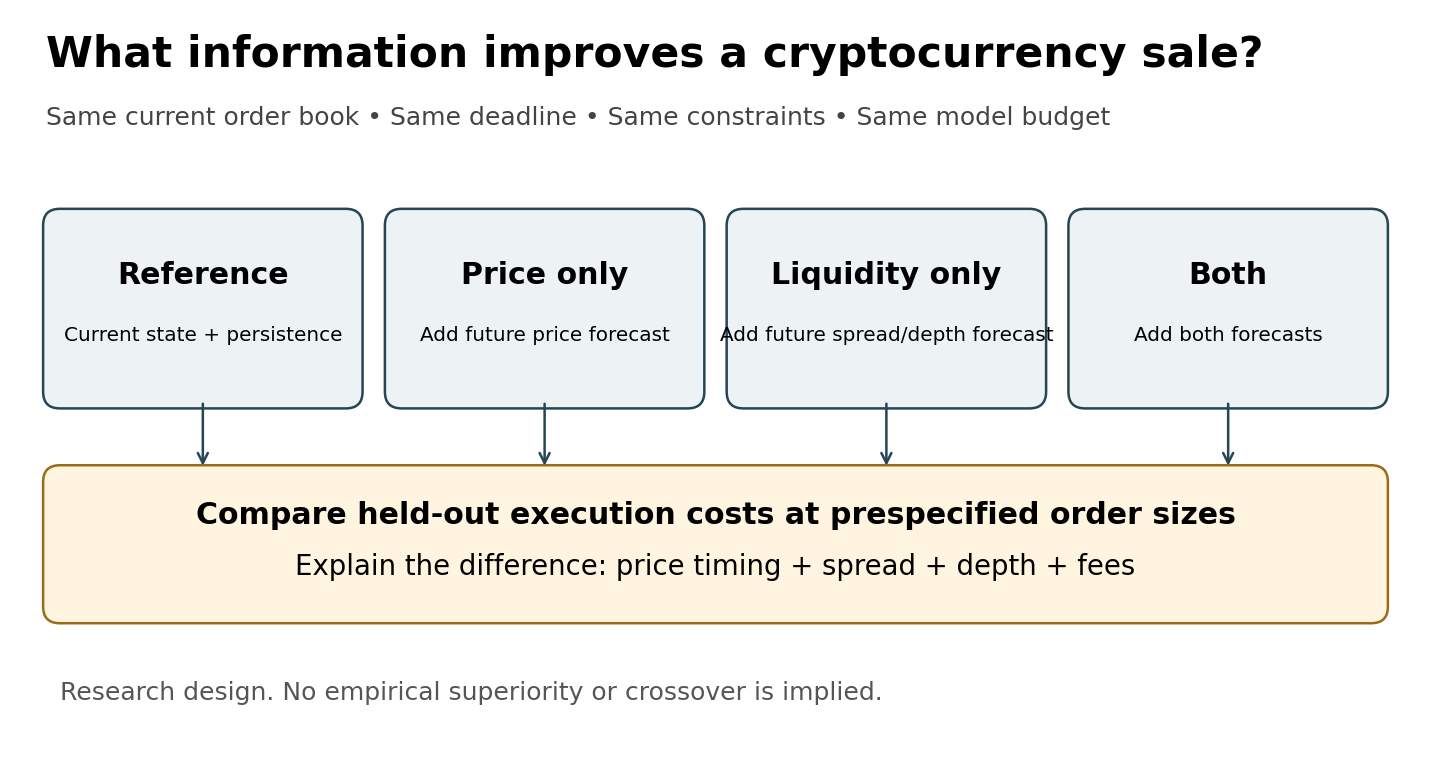
\includegraphics[width=\linewidth]{study_design.png}
\caption{The controlled comparison. This diagram describes the design, not an empirical finding.}
\end{figure}

\section{What existing research already establishes}
Joint price-signal and stochastic-impact execution is established in Fouque, Jaimungal and Saporito \cite{fouque}. Ahabchane and colleagues \cite{ahabchane} forecast book-based transaction costs to improve execution. Kweon, Yim and Min \cite{kweon} train liquidity forecasts for liquidation objectives. Bank, Cartea and K\"orber \cite{bank} compare information about liquidity taking and provision. Consequently, neither combining price and liquidity inputs nor recognising that order size matters is a sufficient novelty claim.

The proposed empirical distinction is the four-arm comparison with shared current information, a credible seasonal reference, fixed forecasting choices and explicit order sizes. The accounting decomposition explains any observed difference. It is not a new theorem. The literature screen does not certify priority: the full Kweon article and other closely related studies still require comparison before final submission wording.

\section{A transparent mechanism}
For intuition, approximate proceeds from selling $Q$ units at time $t$ as
\[
 R_t(Q)=Q(m_t-s_t)-k_tQ^2,
\]
where $m_t$ is the midpoint, $s_t$ the half-spread and $k_t$ the coefficient of total depth cost. If $A$ is the expected increase in price net of spread and $B$ the expected increase in $k$, waiting changes expected proceeds by
\[
 QA-Q^2B.
\]
When $A,B>0$, waiting is preferred in this two-action illustration only below $Q=A/B$. This compares selling entirely now with selling entirely later. It neither proves a crossover for an optimized split schedule nor establishes the value of an imperfect forecast. The empirical size pattern must therefore be allowed to contradict this illustration.

For a completed sale, monetary shortfall has the exact decomposition
\[
 Qm_0-\sum_j R_j+F
 =\sum_jq_j(m_0-m_j)+\sum_jq_j(m_j-b_j)
   +\sum_j(q_jb_j-R_j)+F.
\]
The terms are price-timing shortfall, spread, depth and fees. Their differences reveal whether reduced liquidity costs compensate for changed price exposure.

\section{Pilot design and data}
The public CC0 dataset by Martin S\o gaard Nielsen contains Coinbase BTC, ETH and ADA books \cite{data}. We downloaded approximately 3.09 million one-second records and sampled the latest record available by each UTC minute, rejecting ages above five seconds and invalid books. Source timestamps include a UTC offset, but independently measured receipt and exchange times are unavailable. Fifteen displayed levels are reconstructed from midpoint-relative distances and individual-level notionals. The referenced collector implementation supports these transformations, although the dataset does not pin its precise software version.

The design was recorded before strategy outcomes: train on 8--13 April 2021; evaluate on 14--18 April 2021. Decisions occur at :05 and :35 UTC, with execution over the next fifteen minute boundaries. Valid windows require five preceding observations and fifteen future observations. This produces 691 arrival windows; 685 complete under every policy and order size. Their common support is used for all headline contrasts. Data-quality exclusions depend on subsequent data availability and may limit representativeness.

Each asset uses one ridge specification, with penalty one, training-only standardization and no hyperparameter search. Inputs include lagged returns, spread, depth, imbalance and time of day. Forecasts predict future midpoint changes, half-spread ratios and depth ratios. All arms preserve the same current ladder shape beyond the half-spread. The reference holds price constant and adjusts current spread and depth using a training-only daily seasonal profile. A separate TWAP benchmark is retained.

Parent quantities are 1\%, 5\% and 20\% of displayed bid depth at arrival. At 5\%, the median arrival notional is approximately USD 7,430. The planner maximizes predicted proceeds subject to a child cap of one third of the parent order. Replay walks finite observed depth, carries unsupported quantities forward subject to the same cap, and reports unfinished orders without invented fills. Main replay retains consumed quantity at a price while that price remains observed; independent-snapshot replenishment is a sensitivity. Neither convention captures the market's response to hypothetical orders. Continuous quantities, exchange lot rules, minimum notionals and subsecond latency remain limitations.

\section{Results: the proposed advantage is not established}
Table~\ref{tab:results} reports savings relative to the seasonal current-book reference. Means give equal weight to the five evaluation dates and equal weight to represented assets within each date. Every learned-forecast policy has negative pooled savings at every size. Liquidity forecasts lose less than price forecasts, but that relative advantage narrows as the order grows. The prespecified large-minus-small contrast is $-0.468$ basis points, contrary to the proposed increasing-relative-value hypothesis.

\begin{table}[h]
\centering
\caption{Descriptive savings in basis points; positive means lower cost.}\label{tab:results}
\begin{tabular}{lrrrr}\toprule
Share of depth & Price & Liquidity & Both & Liquidity $-$ price\\\midrule
1\% & $-3.127$ & $-1.525$ & $-3.840$ & $1.601$\\
5\% & $-3.245$ & $-1.861$ & $-3.795$ & $1.384$\\
20\% & $-1.329$ & $-0.196$ & $-1.782$ & $1.134$\\\bottomrule
\end{tabular}
\end{table}

At the 5\% size, liquidity forecasting saves $0.060$ bps in spread and $0.029$ bps in depth costs, but loses $1.950$ bps through price timing. Thus a reduction in the cost of finding buyers is overwhelmed by changed price exposure. This is an interpretable pilot observation; five evaluation dates do not establish its persistence. The largest daily loss is on 18 April, which remains in all reported results.

\begin{figure}[h]
\centering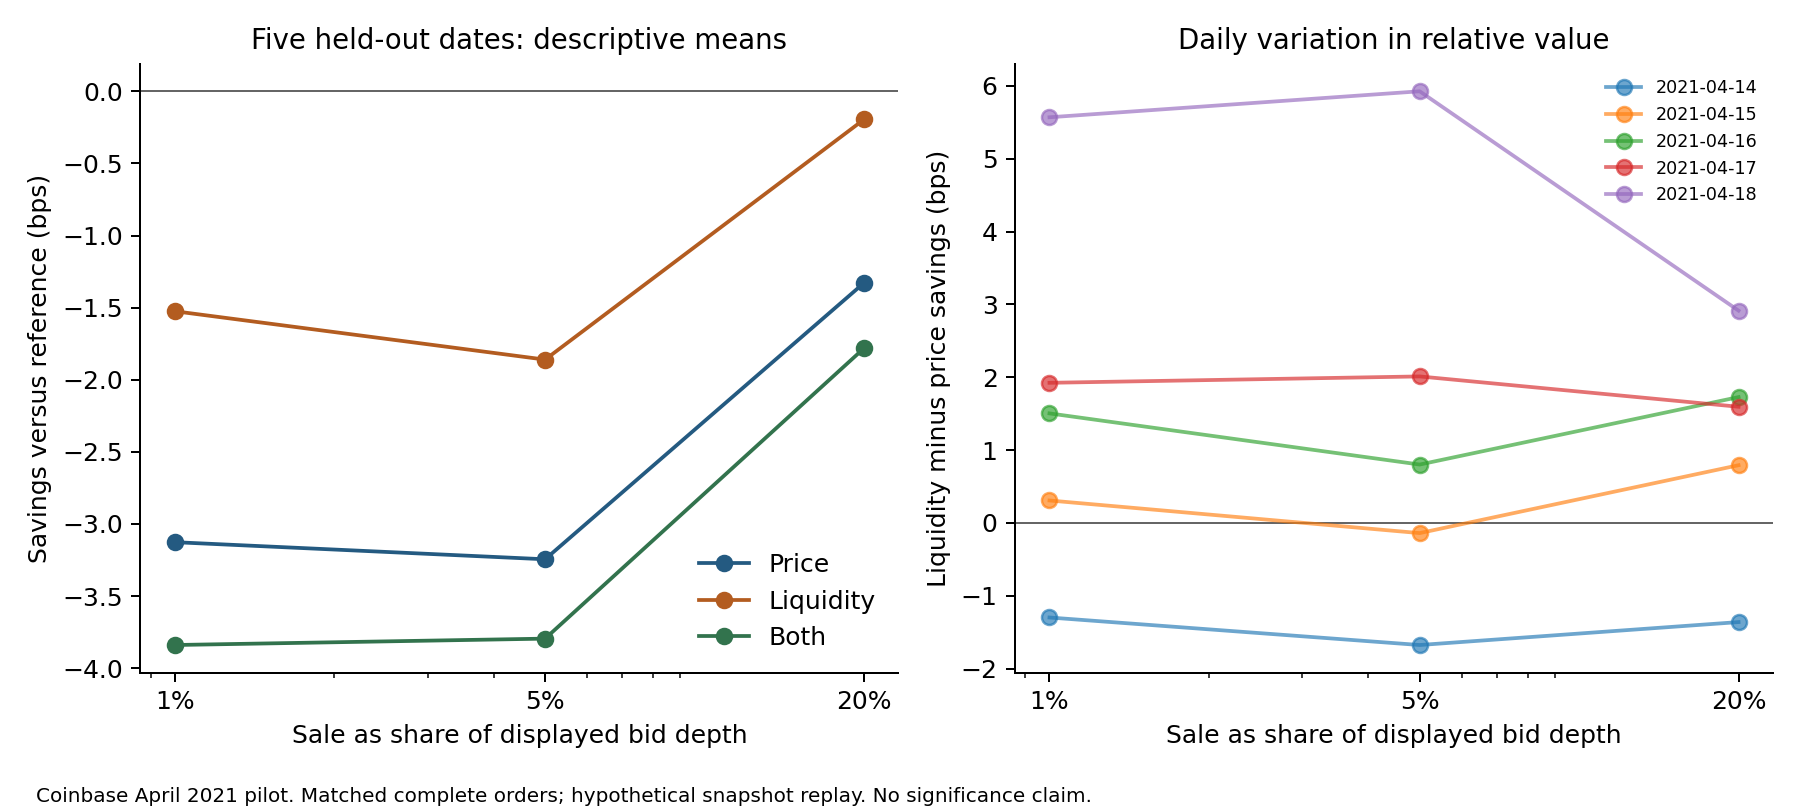
\includegraphics[width=\linewidth]{pilot_information_value.png}
\caption{Pilot means and daily variation. Descriptive pilot; no inferential intervals are reported.}
\end{figure}

The reference also outperforms TWAP by $2.563$ bps at the central size. This is descriptive evidence from the same five dates, not an independently established strategy improvement. At 20\% depth, completion ranges from 99.13\% to 100\% across policies. The prespecified 1\% incompletion guard is not triggered, but six arrivals are excluded from the matched complete sample. All failures remain in the episode records. Independent-snapshot replay produces nearly identical pooled central-size results. A common illustrative 10bps proportional fee scales relative proceeds; it does not rescue the forecast policies.

\section{Was the failure caused by weak forecasts or weak information?}
After completing the frozen pilot, we recorded and ran a separate hindsight diagnostic. It uses the same arrivals and constraints but supplies realized future inputs to the planner. These schedules are not feasible strategies. Only the full oracle is an upper bound within the planner; a single-input hindsight schedule still substitutes the reference for its missing input.

At the 5\% size, supplying the realized future price path saves 25.805 bps, while the full oracle saves 25.850 bps. Realized future books add 0.045 bps after future prices are known. The corresponding increments are 0.033, 0.045 and 0.075 bps as the sale grows from 1\% to 20\% of displayed depth. Thus future price timing dominates the ex-post opportunity in this pilot. Liquidity becomes incrementally more relevant for larger orders, but its magnitude remains small relative to roughly 26--27 bps of price information.

\begin{figure}[h]
\centering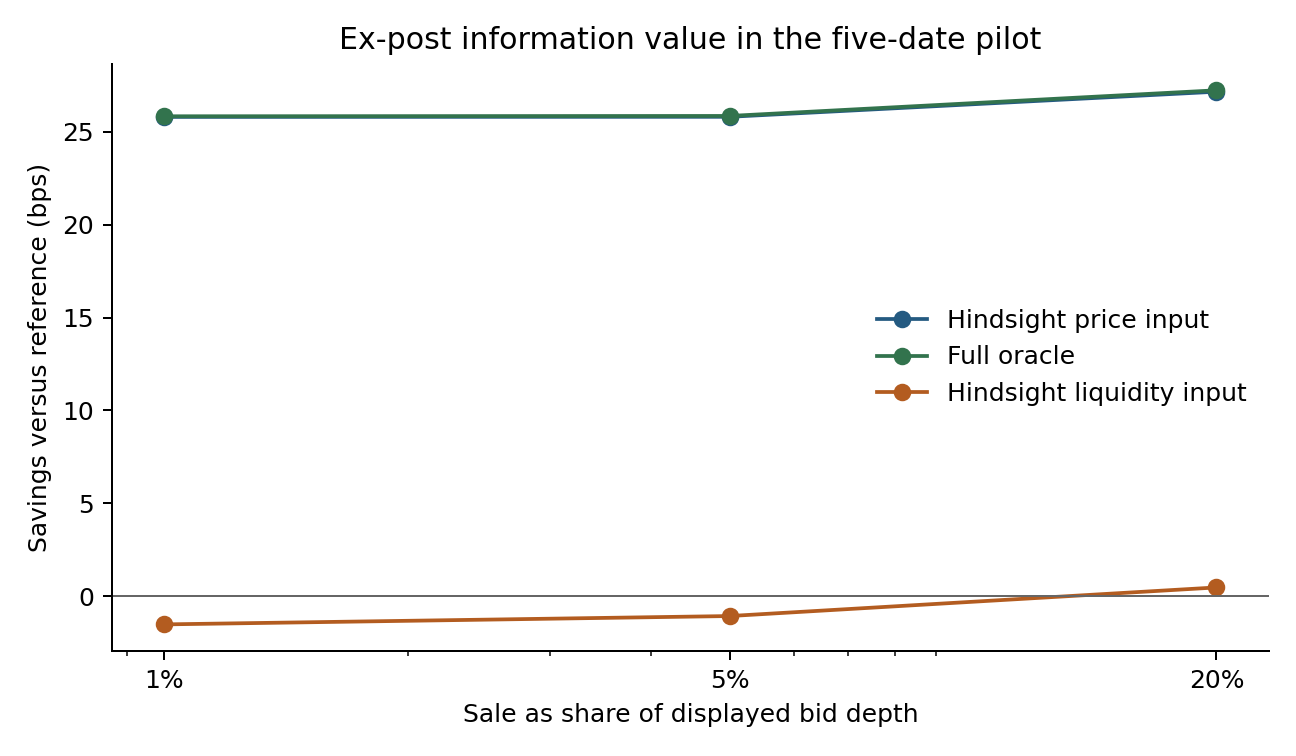
\includegraphics[width=.78\linewidth]{oracle_value.png}
\caption{Post-pilot hindsight diagnostic. Values measure ex-post decision relevance, not achievable forecast performance.}
\end{figure}

The learned price policy loses 3.309 bps at the central size despite the large hindsight-price opportunity. The observed failure therefore cannot be attributed to an absence of price-timing value. The tested causal forecast did not capture that value and shifted execution in the wrong direction on average. Improving this result requires stronger forecasting and policy calibration on new data, not a more favourable description of the existing policy.

\section{Decision and next evidence required}
The contribution is now specific enough to test: quantify the attainable value of price and liquidity information at a given order size, measure how much causal forecasts realize, and show which cost channel explains the difference. The pilot indicates a large unused price-timing opportunity and a small size-dependent liquidity increment. It has not established an effective feasible policy or a stable population relationship. It should not be presented as a stronger completed paper merely because the design is more elaborate.

A larger study needs a substantially longer order-book history, multiple market conditions, stronger validation of execution assumptions and a fresh frozen evaluation period. The closest open historical candidate is the CC0 multi-exchange Bitcoin dataset associated with Hautsch, Scheuch and Voigt \cite{dryad}; its download currently requires access not available in this session. An accessible vendor sample was kept out of the research package because its redistribution and model-use terms conflict with a fully open release. No paid subscription or exchange order was placed.

The present code and data provide a reproducible development platform. Thirteen targeted tests cover allocation, depth accounting, caps, future-data isolation and training boundaries. An isolated rerun verifies the original episode records, fits and forecast-error outputs. Future experiments must be recorded separately; these five dates cannot be reused as untouched confirmation after model changes.

\begin{thebibliography}{9}\small
\bibitem{fouque} Fouque, J.-P., Jaimungal, S., and Saporito, Y. (2022). Optimal Trading with Signals and Stochastic Price Impact. \emph{SIAM Journal on Financial Mathematics}, 13(3), 944--968. \href{https://doi.org/10.1137/21M1394473}{doi:10.1137/21M1394473}.
\bibitem{ahabchane} Ahabchane, Cenesizoglu, Grass, and Jena (2024). Reducing transaction costs using intraday forecasts of limit order book slopes. \emph{Journal of Forecasting}, 43(8), 2982--3008. \href{https://doi.org/10.1002/for.3164}{doi:10.1002/for.3164}.
\bibitem{kweon} Kweon, S., Yim, Y., and Min, S. (2024). Optimizing Sequential Predictions for Order Execution: a Decision Focused Learning Approach. \emph{ICAIF}, 719--727. \href{https://doi.org/10.1145/3677052.3698665}{doi:10.1145/3677052.3698665}.
\bibitem{bank} Bank, P., Cartea, \'A., and K\"orber, L. (2026). Optimal execution and speculation with trade signals. \emph{Finance and Stochastics}. \href{https://doi.org/10.1007/s00780-026-00602-x}{doi:10.1007/s00780-026-00602-x}.
\bibitem{data} Nielsen, M. S. (2021). High Frequency Crypto Limit Order Book Data. Kaggle, CC0. \url{https://www.kaggle.com/datasets/martinsn/high-frequency-crypto-limit-order-book-data}.
\bibitem{dryad} Voigt, S., Hautsch, N., and Scheuch, C. (2024 version). Data from: Building trust takes time: Limits to arbitrage for blockchain-based assets. Dryad, CC0. \href{https://doi.org/10.5061/dryad.q2bvq83rn}{doi:10.5061/dryad.q2bvq83rn}.
\end{thebibliography}
\end{document}
